\documentclass[12pt,a4paper]{article}
\usepackage[utf8]{inputenc}
\usepackage[spanish]{babel}
\usepackage{amsmath}
\usepackage{amsfonts}
\usepackage{amssymb}
\usepackage{graphicx}
\usepackage[left=2cm,right=2cm,top=2cm,bottom=2cm]{geometry}

\usepackage{enumitem}
\usepackage{algorithm}
\usepackage{algorithmic}
\usepackage[hidelinks]{hyperref}

\usepackage{subcaption}
\usepackage{pgfplots}

% Para la tabla
\usepackage{multirow}
\usepackage[normalem]{ulem}
\useunder{\uline}{\ul}{}


\author{Ignacio Aguilera Martos}
\title{Trabajo Integrador \\ Introducción a la Ciencia de Datos}
\date{22 de Diciembre de 2019}

\setlength{\parindent}{0cm}
\setlength{\parskip}{10px}


\begin{document}
	\maketitle

	\tableofcontents

	\newpage
	
\section{Análisis Exploratorio de los Datos}

En esta primera sección vamos a hacer una exploración de los datos intentando extraer algunas conclusiones de los mismos y poder conocer más en profundidad la información que nos arrojan las variables. Esta sección va a estar dividida en dos subsecciones, una para el conjunto de regresión y otra para el conjunto de clasificación.

\subsection{Conjunto de Regresión}

El conjunto de datos del que dispongo para realizar regresión es el conjunto ``treasury''. Vamos a analizar el conjunto de datos.

En primer lugar el conjunto de datos dispone de  16 variables numéricas como podemos observar con el siguiente código.

\begin{figure}[H]
	\centering
	\begin{subfigure}{0.47\textwidth}
		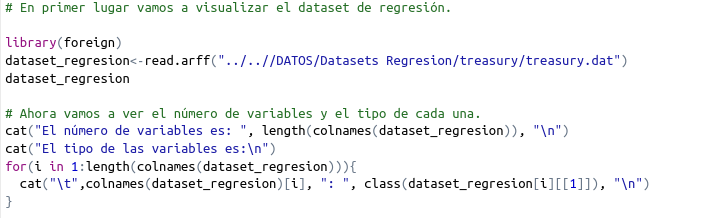
\includegraphics[scale=0.35]{./Imagenes/EDA/Regresion/codigo_variables_tipos.png}
	\end{subfigure}
	\begin{subfigure}{0.47\textwidth}
		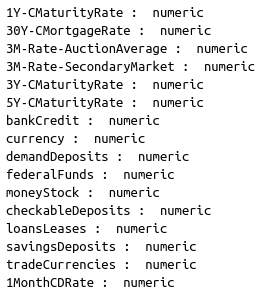
\includegraphics[scale=0.4]{./Imagenes/EDA/Regresion/variables_tipos.png}
	\end{subfigure}
	\caption{Tipos de las variables y código para obtenerlos}
\end{figure}

Como podemos ver el conjunto dispone de 16 variables de las cuales todas son numéricas. Esto es lógico pues el conjunto está destinado para el problema de regresión y además nos facilita el trabajo. 

Para poder seguir analizando el conjunto vamos a hacer un estudio pormenorizado de las variables del mismo en función a una serie de estadísticos básicos.

Estos estadísticos que voy a emplear son: media, mediana, moda, desviación típica, mínimo, máximo, curtosis y asimetría.

En este conjunto podemos dividir las variables en dos grupos. El primero de ellos corresponde a las variables de entrada que son las que nos van a permitir obtener resultados sobre la salida y el segundo grupo es la propia salida esperada del sistema.

Vamos a empezar a analizar en primer lugar la salida.

\subsubsection{Estudio de los estadísticos}

\subsubsection*{Salida}
La variable de salida es la que tiene por nombre 1MonthCDRate. Los estadísticos que nos arroja esta variable son los siguientes:

\begin{figure}[H]
	\centering
	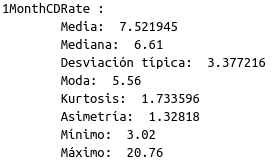
\includegraphics[scale=0.7]{./Imagenes/EDA/Regresion/estadisticos_1MonthCDRate.png}
	\caption{Estadísticos de la variable de salida.}
\end{figure}

Podemos observar que la  media de la salida es aproximadamente de $7.5$ y su desviación típica de $3.3$, esto nos indica que la mayoría de los datos (el 95\% en caso de estar ante una distribución normal) van a estar dentro del intervalo $[0.9,14,1]$. Aún así podemos ver mediante el mínimo y el máximo que los datos se van a mover en el intervalo $[3.02, 20.76]$. Esto parece que nos va a indicar que deberíamos de tener una cola más pesada a la izquierda de la distribución y una cola más alargada a la derecha de la misma. Este hecho viene corroborado también por la mediana. Vemos que es $6.61$ (menor que la media) con lo que nos está diciendo que el 50\% de los datos van a estar en el intervalo $[3.02, 6.61]$ y por tanto proporcionalmente esta cola será más pesada.

Otra forma que tenemos de comprobar lo que hemos dicho es mediante el coeficiente de asimetría. Al ser positivo nos está indicando que la distribución es asimétrica a la derecha, cuestión que ya sabemos y hemos razonado.

La curtosis nos está dando una indicación de cómo de puntiaguda o achatada es la distribución. En este caso el coeficiente es positivo, por lo que la distribución será más puntiaguda. Esto nos está indicando que vamos a tener una mayor concentración de datos entorno a la media.

\subsubsection*{Variable 1: 1Y-CMaturityRate}

Los estadísticos que nos arroja esta variable son:

\begin{figure}[H]
	\centering
	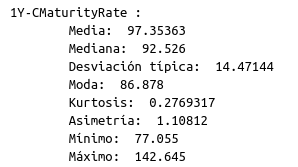
\includegraphics[scale=0.7]{./Imagenes/EDA/Regresion/estadisticos_1Y_CMaturityRate.png}
	\caption{Estadísticos de la variable 1 1Y\_CMaturityRate}
\end{figure}

En primer lugar podemos observar que la media es de $97.35363$ y la mediana es ligeramente inferior. Esto nos vuelve a indicar que vamos a tener una cola más corta a la izquierda y una más larga a la derecha, es decir, vamos a tener más valores a la derecha de la distribución. Podemos corroborar este hecho también comprobando el mínimo y el máximo. Como podemos ver el máximo está mucho más alejado de la media que el mínimo por lo que podemos intuir que la distribución va a ser más alargada por ese lado.

De igual forma si miramos el coeficiente de asimetría vemos que es positivo lo que nos está indicando la asimetría de la cola derecha.

La curtosis es positiva pero no muy lejana del cero, por lo que tendrá la forma de una normal pero un poco más puntiaguda.

\subsubsection*{Variable 2: 30Y-CMortgageRate}

Los estadísticos que nos arroja esta variable son:

\begin{figure}[H]
	\centering
	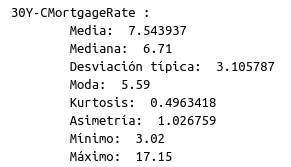
\includegraphics[scale=0.7]{./Imagenes/EDA/Regresion/estadisticos_30Y_CMortgageRate.png}
	\caption{Estadísticos de la variable 2 30Y\_CMortgageRate}
\end{figure}

Podemos ver que la media es $7.543937$ y la mediana $6.71$ lo que de nuevo nos hace sospechar que la cola derecha es más alargada. Esto lo podemos ver (y podemos decir ya que la cola va a ser bastante alargada) con el máximo y el mínimo. Sabemos que el 95\% de los datos debería de estar en el intervalo $[ media-2*stdv, media+2*stdv ]$ pero la realidad es que observamos que la cola derecha es más larga. Asimismo vemos que la moda es aún menor que la mediana con lo que corroboramos que la cola izquierda es más pesada y la derecha más alargada.

El coeficiente de asimetría nos termina de corroborar lo que estamos infiriendo pues al ser positivo nos indica una asimetría en la cola derecha.

En cuanto a la curtosis podemos ver que es más puntiaguda que una normal.

\subsubsection*{Variable 3: 3M-Rate-AuctionAverage}

Los estadísticos que nos arroja esta variable son:

\begin{figure}[H]
	\centering
	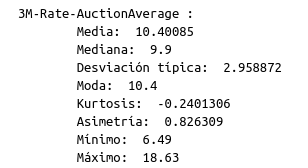
\includegraphics[scale=0.7]{./Imagenes/EDA/Regresion/estadisticos_3M_Rate_AuctionAverage.png}
	\caption{Estadísticos de la variable 3 3M\_Rate\_AuctionAverage}
\end{figure}

Esta variable tiene como media $10.40085$ y mediana $9.9$. En esta variable no vemos una diferencia tan grande por lo que a priori podemos pensar que no es muy asimétrica. La desviación típica es de $2.958872$ por lo que (en caso de que fuese una normal) el 95\% de los datos se van a encontrar en el intervalo $[4.483106, 16.318594]$. Vemos que el mínimo es $6.49$ con lo que podemos entender que la cola izquierda es más corta mientras que el máximo es $18.63$ con lo que la cola derecha va a ser algo más alargada.

Si observamos los coeficiente de asimetría y curtosis podemos ver que el coeficiente de asimetría es positivo lo que nos indica que la distribución es asimétrica a la derecha y la curtosis es ligeramente negativa con lo que podemos decir que la distribución será algo más achatada que una distribución normal.

\subsubsection*{Variable 4: 3M-Rate-SecondaryMarket}

Los estadísticos que nos arroja esta variable son:

\begin{figure}[H]
	\centering
	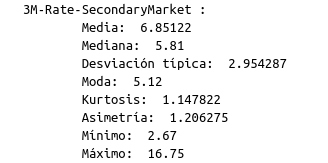
\includegraphics[scale=0.7]{./Imagenes/EDA/Regresion/estadisticos_3M_Rate_SecondaryMarket.png}
	\caption{Estadísticos de la variable 4 3M\_Rate\_SecondaryMarket}
\end{figure}

Podemos observar que el comportamiento de esta variable es el mismo que las anteriores y que va a tener una cola a la derecha más alargada. Esto es comprobable por todas las razones expuestas en las secciones anteriores.

\subsubsection*{Variable 5: 3Y-CMaturityRate}

Los estadísticos que nos arroja esta variable son:

\begin{figure}[H]
	\centering
	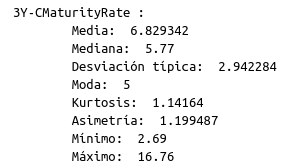
\includegraphics[scale=0.7]{./Imagenes/EDA/Regresion/estadisticos_3Y_CMaturityRate.png}
	\caption{Estadísticos de la variable 5 3Y\_CMaturityRate}
\end{figure}

De igual forma los estadísticos de esta variable nos están arrojando la misma información que para el resto de variables con una cola derecha muy alargada. Podemos corroborar esta información por lo mismo que hemos dicho antes (mediana, media, máximo y míninimo) además de coeficiente de asimetría que al ser positivo nos indica que es asimétrica a la derecha.

Por otro lado, al igual que en los casos previos, la curtosis nos indica que la distribución es más puntiaguda o apuntada que una distribución normal.

\subsubsection*{Variable 6: 5Y-CMaturityRate}

Los estadísticos que nos arroja esta variable son:

\begin{figure}[H]
	\centering
	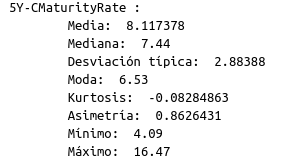
\includegraphics[scale=0.7]{./Imagenes/EDA/Regresion/estadisticos_5Y_CMaturityRate.png}
	\caption{Estadísticos de la variable 6 5Y\_CMaturityRate}
\end{figure}

En esta variable observamos también una cola derecha más alargada pero podemos observar que aquí no es una cola tan alargada como en los casos anteriores. 

Si comprobamos la media y la mediana observamos que la mediana es menor que la media por lo que ya nos está apuntando a la asimetría pero si vemos la desviación típica y calculamos el intervalo en el que deberían estar el 95\% de los datos ($[2.349618, 13,885138]$) podemos percibir que la cola izquierda es más corta (pues el mínimo es $4.09$) y la cola derecha más alargada pues el máximo llega hasta $16.47$.

Podemos decir que la asimetría derecha se manifiesta pero con menor intensidad como podemos percibir por el coeficiente de asimetría, pues aunque es positivo, es menor que en otros casos.

En cuanto a la curtosis podemos ver que es ligeramente negativa pero muy cercana al cero por lo que podemos decir que la distribución esta ligerísimamente achatada con respecto a una normal aunque visualmente probablemente no pudiéramos distinguirlo.

\subsubsection*{Variable 7: bankCredit}

Los estadísticos que nos arroja esta variable son:

\begin{figure}[H]
	\centering
	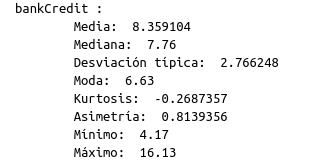
\includegraphics[scale=0.7]{./Imagenes/EDA/Regresion/estadisticos_bankCredit.png}
	\caption{Estadísticos de la variable 7 bankCredit}
\end{figure}

En este caso podemos ver que la mediana es más pequeña que la media por lo que podemos pensar de nuevo en que esta variable tiene una cola derecha más alargada. Si calculamos el intervalo en el que deberían de estar el 95\% de los datos ($[2.826608,13.8916]$) podemos apreciar esa tendencia a una cola derecha más pesada. 

Aún así, si comprobamos el coeficiente de asimetría, podemos ver que se manifiesta la asimetría derecha pero de forma ligera como en la variable anterior pues el coeficiente no es tan grande como en otras variables que ya hemos analizado. 

En cuanto a la curtosis tenemos una curtosis negativa lo que nos indica que la distribución está algo más achatada que su correspondiente distribución normal.

\subsubsection*{Variable 8: currency}

Los estadísticos que nos arroja esta variable son:

\begin{figure}[H]
	\centering
	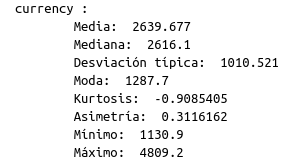
\includegraphics[scale=0.7]{./Imagenes/EDA/Regresion/estadisticos_currency.png}
	\caption{Estadísticos de la variable 8 currency}
\end{figure}

En este caso la mediana también es algo más pequeña que la media, pero si comprobamos el rango de valores de la variable ($[1130.9, 4809.2,]$) observamos que la diferencia no es tan significativa por lo que no podemos decir tan rápido que tenemos una cola derecha más alargada. Como vemos la desviación típica es de $1010.521$ por lo que el intervalo que debe contener el 95\% de los datos es $[618.635,4660,719]$. 

Con esta información podemos apuntar que debe existir una ligera asimetría en la cola derecha porque el mínimo es mayor que el mínimo que nos da el intervalo del 95\% de los datos y el máximo es algo mayor que el máximo del intervalo del 95\%.

Para contrastar esta información tenemos el coeficiente de asimetría que, al ser positivo, nos dice que la distribución presenta asimetría derecha pero podemos ver que es mucho más pequeño que en el resto de variables con lo que la asimetría no es tan pronunciada.

En cuanto a la curtosis podemos ver que es negativa por lo que la distribución es más achatada que una distribución normal.

\subsubsection*{Variable 9: demandDeposits}

Los estadísticos que nos arroja esta variable son:

\begin{figure}[H]
	\centering
	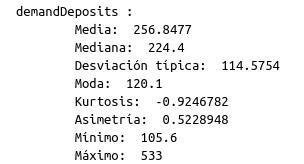
\includegraphics[scale=0.7]{./Imagenes/EDA/Regresion/estadisticos_demandDeposits.png}
	\caption{Estadísticos de la variable 9 demandDeposits}
\end{figure}

Como podemos observar tenemos que la mediana es menor que la media. Volvemos a tener una situación que nos lleva a pensar que tenemos una cola derecha más alargada que la izquierda.

Si calculamos el intervalo en el que debe estar el 95\% de los datos ($[27.6969,485.9985]$) podemos observar que el máximo es algo más grande que el máximo de dicho intervalo e igualmente ocurre con el mínimo con lo que tenemos un desplazamiento de los datos hacia la derecha.

El hecho viene refrendado por el coeficiente de asimetría que al ser positivo nos indica dicha asimetría derecha.

En cuanto a la curtosis al tener una curtosis negativa estamos ante una distribución más achatada que en el caso de una normal.

\subsubsection*{Variable 10: federalFunds}

Los estadísticos que nos arroja esta variable son:

\begin{figure}[H]
	\centering
	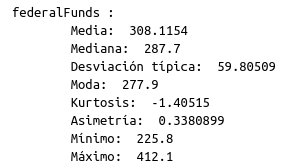
\includegraphics[scale=0.7]{./Imagenes/EDA/Regresion/estadisticos_federalFunds.png}
	\caption{Estadísticos de la variable 10 federalFunds}
\end{figure}

Podemos observar en esta variable el mismo comportamiento que venimos destacando del resto. Tenemos que la mediana es más pequeña que la media lo que nos indica que la cola derecha de la distribución debe ser algo más alargada.

El intervalo en el que el 95\% de los datos debe caer es $[188.50522, 427.72558]$. Podemos ver que el máximo de este intervalo es ligeramente más grande que el máximo y el mínimo es ligeramente más grande que el del intervalo del 95\% por lo que podemos decir que si existe una asimetría derecha esta no es muy pronunciada.

Podemos contrastar lo que estamos afirmando por el coeficiente de asimetría que es ligeramente positivo, por lo que se confirma lo que estamos razonando de que tenemos una ligera asimetría derecha.

En cuanto a la curtosis tenemos que es negativa y grande por lo que será muy achatada con respecto a una normal de mismos parámetros.

\subsubsection*{Variable 11: moneyStock}

Los estadísticos que nos arroja esta variable son:

\begin{figure}[H]
	\centering
	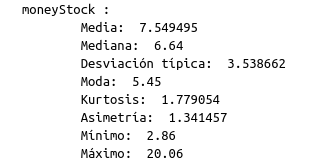
\includegraphics[scale=0.7]{./Imagenes/EDA/Regresion/estadisticos_moneyStock.png}
	\caption{Estadísticos de la variable 11 moneyStock}
\end{figure}

Podemos repetir exactamente el mismo razonamiento que hemos hecho anteriormente para argumentar la asimetría derecha, pero en este caso al comprobar el coeficiente de asimetría podemos ver que es mucho más pronunciada.

En cuanto a la curtosis tenemos el comportamiento opuesto al de la variable anterior teniendo que la distribución es significativamente más puntiaguda o apuntada que su normal de mismos parámetros.

\subsubsection*{Variable 12: moneyStock}

Los estadísticos que nos arroja esta variable son:

\begin{figure}[H]
	\centering
	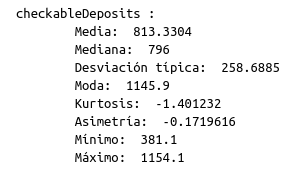
\includegraphics[scale=0.7]{./Imagenes/EDA/Regresion/estadisticos_checkableDeposits.png}
	\caption{Estadísticos de la variable 12 checkableDeposits}
\end{figure}

Este es el primer ejemplo en el que podemos ver como la cola más alargada no va a ser la cola derecha sino la izquierda. En este caso, al igual que los anteriores, podemos ver que la mediana es menor que la media (aunque no mucho proporcionalmente al rango de valores que se toman). Esto podría indicarnos que la cola derecha continúa siendo algo más alargada que la izquierda, pero en este caso podemos apreciar que la moda (el valor más frecuente) es significativamente más grande que la media, por lo que no podemos intuir un comportamiento a priori. Tenemos información contradictoria, una parte nos dice que debemos tener la cola derecha más alargada y la otra nos está diciendo que la izquierda es la que debería ser más alargada.

Para poder estudiar esta situación compleja recurrimos al coeficiente de asimetría. Como podemos ver en este caso es negativo pero ligeramente. Tal y como podíamos pensar la situación está razonablemente equilibrada aunque mostrando una ligera asimetría izquierda.

En cuanto a la curtosis tenemos que es negativa y grande, por lo que estamos ante una distribución mucho más achatada que una distribución normal de mismos parámetros.

\subsubsection*{Variable 13: savingsDeposits}

Los estadísticos que nos arroja esta variable son:

\begin{figure}[H]
	\centering
	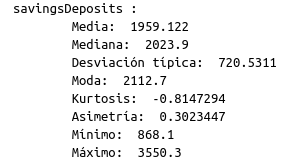
\includegraphics[scale=0.7]{./Imagenes/EDA/Regresion/estadisticos_savingsDeposits.png}
	\caption{Estadísticos de la variable 13 savingsDeposits}
\end{figure}

El caso de esta variable es singular también. Podemos ver que la mediana es mayor que la media, la moda también por lo que podríamos pensar que la cola más alargada es la izquierda. 

Por contra si miramos el intervalo míninimo y máximo podemos ver que lo más probable es que se extienda más la cola derecha pues el máximo es más grande proporcionamente a la media que el mínimo. 

Para contrastar la información miramos el coeficiente de asimetría y observamos que, aunque es pequeño, es positivo. Esto nos indica que la distribución es asimétrica derecha.

Si analizamos la curtosis podemos ver que es negativa lo que nos indica que la distribución es más achatada que una normal de mismos parámetros.

\subsubsection*{Variable 14: tradeCurrencies}

Los estadísticos que nos arroja esta variable son:

\begin{figure}[H]
	\centering
	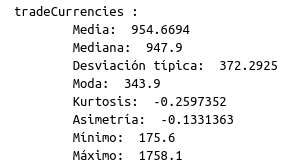
\includegraphics[scale=0.7]{./Imagenes/EDA/Regresion/estadisticos_tradeCurrencies.png}
	\caption{Estadísticos de la variable 14 tradeCurrencies}
\end{figure}

En cuanto a esta variable podemos ver que la media es mayor (ligeramente) que la mediana y la moda es mucho menor que la media. Por contra tenemos que el mínimo es más significativo que el máximo en cuanto al intervalo de valores se refiere. En ese caso a priori no podemos decir nada.

Si miramos el coeficiente de asimetría podemos contrastar esta información pues es muy cercano a cero y en este caso ligeramente negativo por lo que si podemos decir algo es que es ligeramente asimétrica la distribución a la izquierda.

La curtosis es ligeramente negativa por lo que podemos decir que es un poco más achatada que su normal asociada.

\subsubsection{Estudio de la correlación de las variables}

En esta sección vamos a estudiar la correlación entre variables que no son de salida y de dichas variables con la de salida para intentar ver cuales van a ser las más relevantes para nuestro estudio o si hay alguna variable que podamos quitar.

En primer lugar vamos a hacer un estudio de la correlación entre las variables. Nuestro objetivo va a ser obtener aquellas que tienen alta correlación con otras variables, es decir, obtener aquellas variables que son explicadas por otras pues estas las podremos quitar.

Por supuesto todo este estudio habrá que contrastarlo sobre los resultados de la regresión, pero podemos hacer hipótesis previas al ajuste de los modelos.

El código que voy a emplear para el estudio es el siguiente:

\begin{figure}[H]
	\centering
	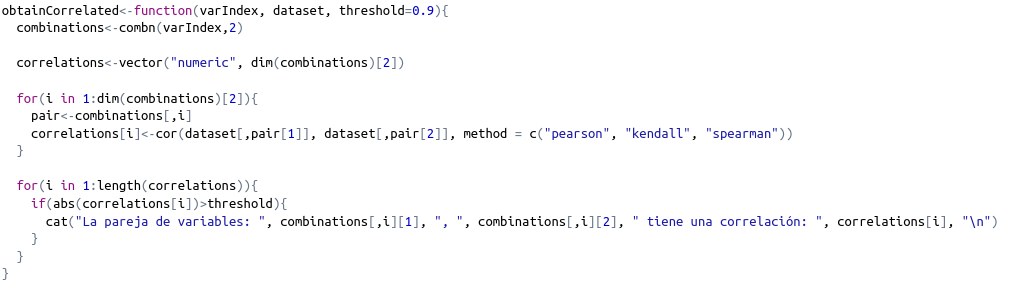
\includegraphics[scale=0.51]{./Imagenes/EDA/Regresion/correlacion_entre_variables_codigo.png}
	\caption{Código para el estudio de la correlación entre variables.}
\end{figure}

Para poder eliminar una variable de forma que estemos seguros de que no quitamos información debemos exigir que la correlación entre variables sea alta. En este caso como se puede ver en el código solamente vamos a mostrar las parejas de variables que presenten una correlación alta, en concreto que en valor absoluto sea mayor a $0.9$.

Vamos a ver las parejas de variables que cumplen esta condición.

\begin{figure}[H]
	\centering
	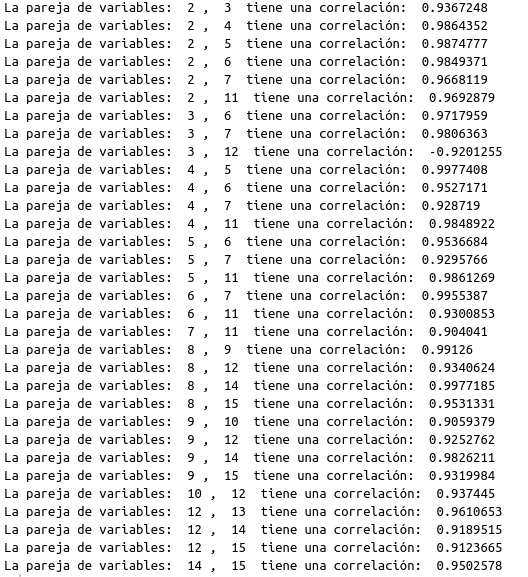
\includegraphics[scale=0.6]{./Imagenes/EDA/Regresion/correlacion_entre_variables1.png}
	\caption{Primer filtrado de la correlación entre variables}
\end{figure}

Podemos observar claramente que la variable 2 tiene una correlación muy alta con otras variables, por lo que podemos eliminarla al ser explicada por las variables 3,4,5,6,7 y 11.

\begin{figure}[H]
	\centering
	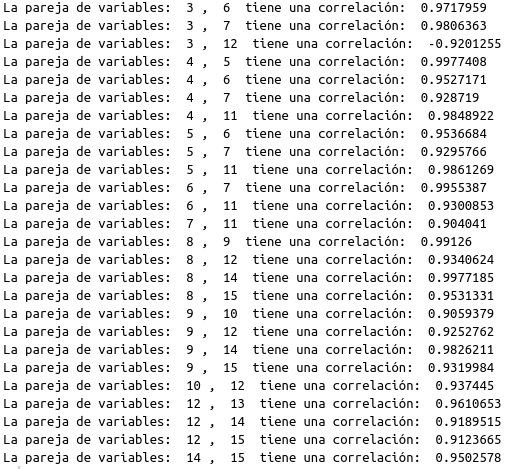
\includegraphics[scale=0.6]{./Imagenes/EDA/Regresion/correlacion_entre_variables2.png}
	\caption{Correlación entre variables después de eliminar la segunda.}
\end{figure}

Podemos ver a su vez que la variable 9 tiene una correlación muy alta con las variables 10, 12, 14 y 15 por lo que podemos eliminarla.

\begin{figure}[H]
	\centering
	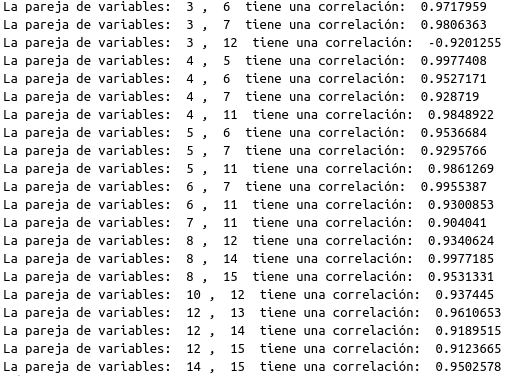
\includegraphics[scale=0.6]{./Imagenes/EDA/Regresion/correlacion_entre_variables3.png}
	\caption{Correlación entre variables después de eliminar la segunda y la novena.}
\end{figure}

La variable 4 podemos ver que tiene alta correlación con las variables 5,6,7 y 11 por lo que podemos quitarla también.

\begin{figure}[H]
	\centering
	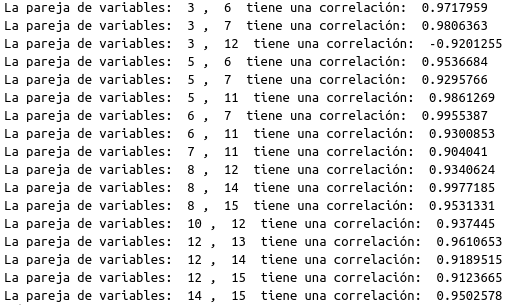
\includegraphics[scale=0.6]{./Imagenes/EDA/Regresion/correlacion_entre_variables4.png}
	\caption{Correlación entre variables después de eliminar la segunda, la novena y la cuarta.}
\end{figure}

La tercera variable sigue manteniendo una alta correlación con las variables 6,7 y 12, por lo que podemos eliminarla.

\begin{figure}[H]
	\centering
	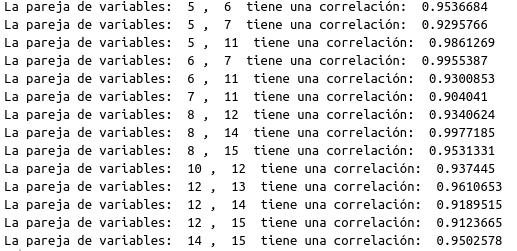
\includegraphics[scale=0.6]{./Imagenes/EDA/Regresion/correlacion_entre_variables5.png}
	\caption{Correlación entre variables después de eliminar la segunda, la novena, la cuarta y la tercera.}
\end{figure}

Podemos ver que la variable 12 y 5 tienen una alta correlación con otras tres que además  no se comparten por lo que podemos eliminar también ambas variables.

\begin{figure}[H]
	\centering
	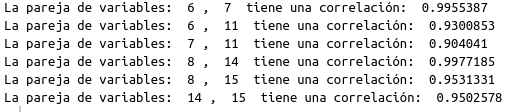
\includegraphics[scale=0.6]{./Imagenes/EDA/Regresion/correlacion_entre_variables6.png}
	\caption{Correlación entre variables después de eliminar la segunda, la novena, la cuarta, la tercera, la duodécima y la quinta.}
\end{figure}

Podemos observar que la variable 6 y 8 tienen alta correlación con otras dos variables no compartidas, por lo que podemos eliminar ambas.

\begin{figure}[H]
	\centering
	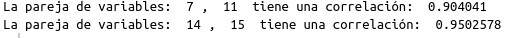
\includegraphics[scale=0.6]{./Imagenes/EDA/Regresion/correlacion_entre_variables7.png}
	\caption{Correlación entre variables después de eliminar la segunda, la novena, la cuarta, la tercera, la duodécima, la quinta, la sexta y la octava.}
\end{figure}

Finalmente nos hemos quedado con dos parejas únicamente por lo que ya no está tan claro la  eliminación de dichas variables. Vamos a parar por tanto el proceso de eliminación en este punto.

Veamos la correlación entre variables que nos queda con las que hemos decidido mantener.

\begin{figure}[H]
	\centering
	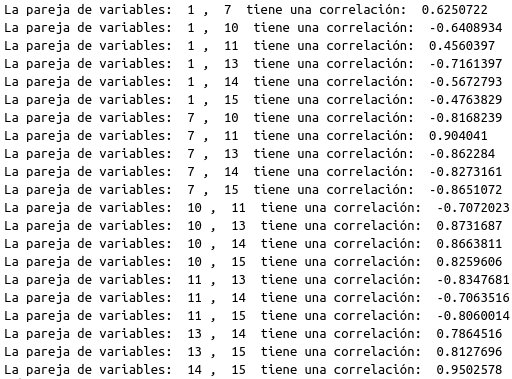
\includegraphics[scale=0.6]{./Imagenes/EDA/Regresion/correlacion_entre_variables8.png}
	\caption{Correlación entre variables después de hacer la limpieza de variables.}
\end{figure}

Finalmente por tanto nos hemos quedado con las variables 1,7,10,11,13,14 y 15.

Sobre estas variables merece la pena estudiar su correlación con la variable de salida para ver que seguimos teniendo variables que explican el comportamiento de la salida.

\begin{figure}[H]
	\centering
	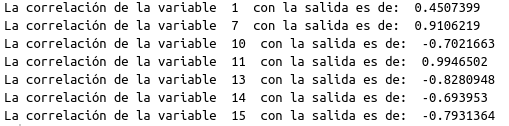
\includegraphics[scale=0.6]{./Imagenes/EDA/Regresion/correlacion_variable_salida1.png}
	\caption{Correlación de las variables no eliminadas con la variable de salida.}
\end{figure}

Podemos ver que las variables 7, 11, 13 y 15 tienen una correlación en valor absoluto mayor a $0.75$ con lo que estas variables nos van a resultar de mucho interés a la hora de realizar un modelo de regresión lineal.

Todas estas hipótesis serán contrastadas en la sección de regresión al ajustar los modelos.

\subsubsection{Valores perdidos}

En cuanto a los valores perdidos vamos a comprobar en primer lugar si tenemos valores NA.

\begin{figure}[H]
	\centering
	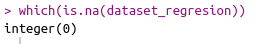
\includegraphics[scale=0.6]{./Imagenes/EDA/Regresion/valores_perdidos.png}
	\caption{Código y resultados para comprobar si tenemos valores perdidos.}
\end{figure}

Como podemos comprobar no tenemos ningún valor perdido.

\subsubsection{Outliers}

Vamos a comprobar si tenemos outliers en nuestro conjunto de datos.

En primer lugar vamos a ver un pairplot de las variables para ver si podemos distinguir algo visualmente.

\begin{figure}[H]
	\centering
	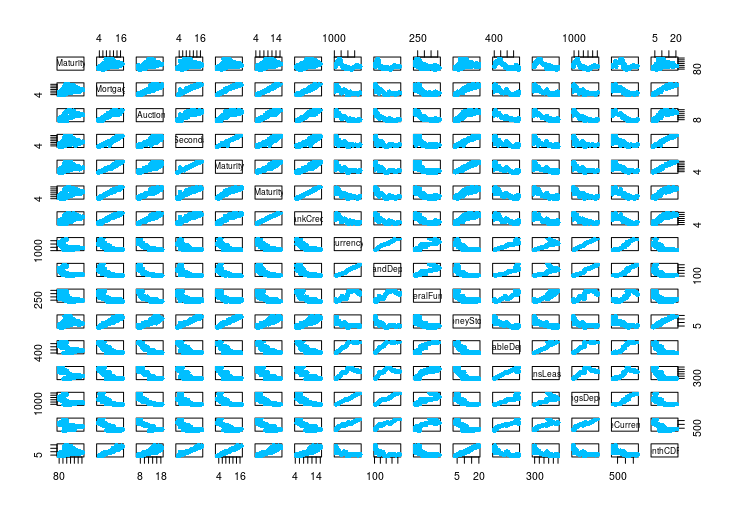
\includegraphics[scale=0.95]{./Imagenes/EDA/Regresion/pairplot_todas.png}
	\caption{Scatterplot de todas las variables dos a dos}
\end{figure}

Visualmente con tantas variables no podemos destacar ninguna anomalía. Vamos a centrarnos solamente en las variables que hemos decidido quedarnos del estudio previo.

\begin{figure}[H]
	\centering
	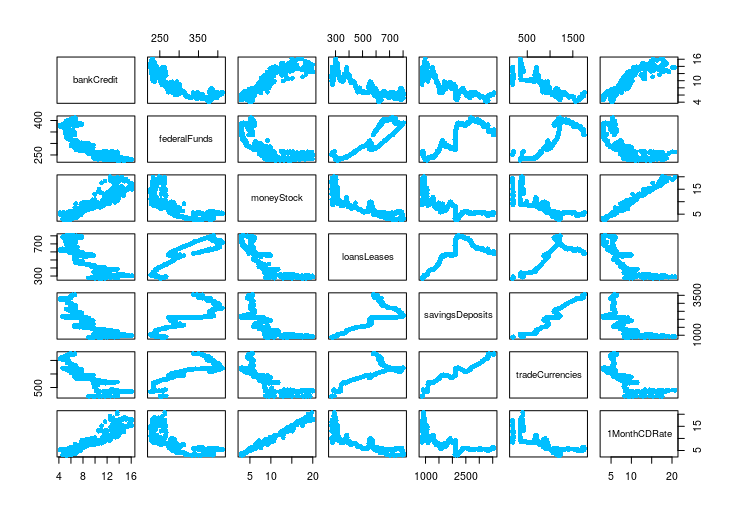
\includegraphics[scale=0.95]{./Imagenes/EDA/Regresion/pairplot_variables_seleccionadas.png}
	\caption{Scatterplot de las variables seleccionadas}
\end{figure}

Como podemos ver no podemos destacar ningún outlier en el conjunto de datos de forma visual.

De paso podemos ver que hemos hecho una selección de variables adecuada pues podemos observar una clara relación lineal con la salida.

Vamos a ver ahora un boxplot de todas las variables.

\begin{figure}[H]
	\centering
	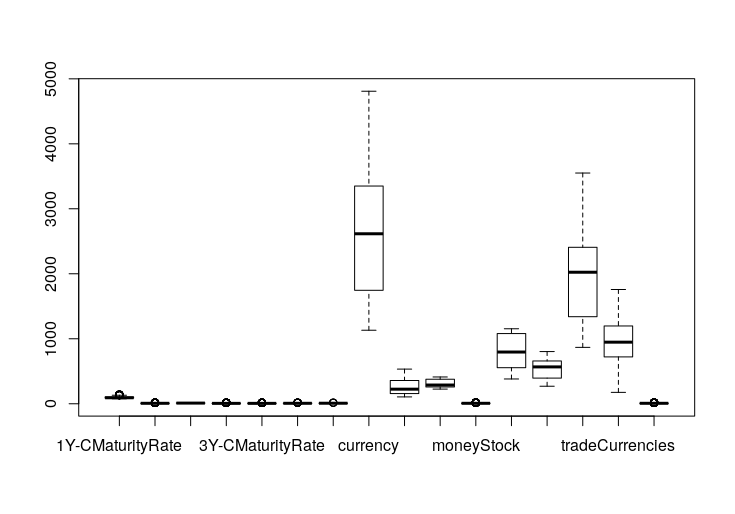
\includegraphics[scale=0.8]{./Imagenes/EDA/Regresion/boxplot_todas.png}
	\caption{Boxplot de las todas las variables}
\end{figure}

Podemos ver que por la diferencia de escalas no todas las variables son visibles. En las que podemos observar de forma adecuada podemos ver que no hay outliers que nos destaquen fuera del rango intercuartil. Por tanto podemos eliminarlas del boxplot para reducir la escala y poder ver el resto de variables.

Para el siguiente boxplot vamos a quitar las variables 8, 9, 10, 12, 13, 14 y 15.

\begin{figure}[H]
	\centering
	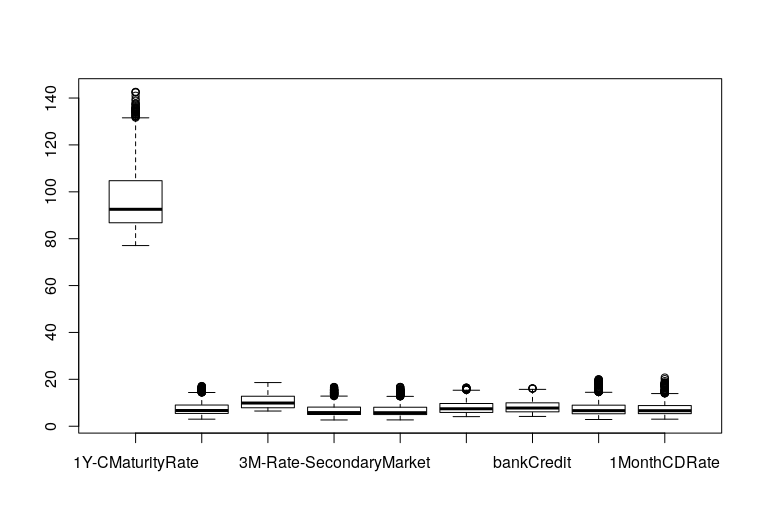
\includegraphics[scale=0.8]{./Imagenes/EDA/Regresion/boxplot_filtrado1.png}
	\caption{Boxplot quitando las variables 8, 9, 10, 12, 13, 14 y 15}
\end{figure}

Podemos observar que la primera variable tiene una escala mayor que el resto, por lo que para poder continuar la tendremos que quitar. Si observamos sus valores podemos ver que tenemos algunas anomalías por encima. Al tener tantos valores por encima no podemos decir de forma tan clara que estos valores son anómalos pues podría ser un comportamiento esperado de la variable y por tanto a priori no debemos eliminar dichos valores.

Eliminamos además la variable 1 para continuar con el estudio.

\begin{figure}[H]
	\centering
	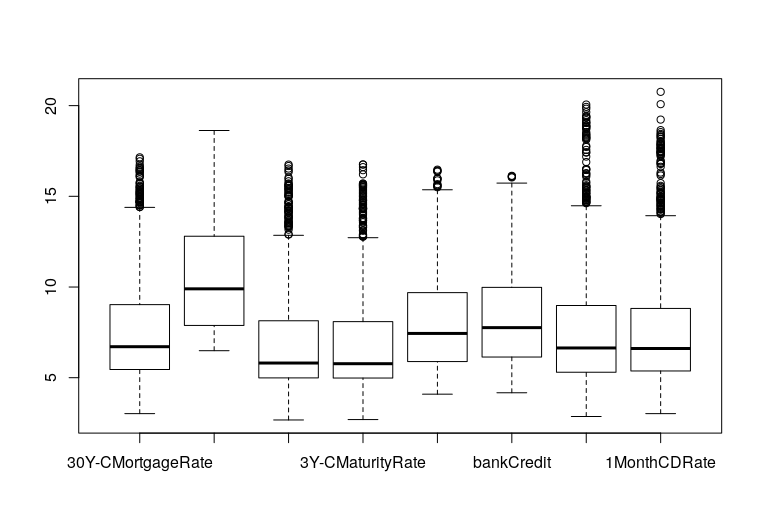
\includegraphics[scale=0.8]{./Imagenes/EDA/Regresion/boxplot_filtrado2.png}
	\caption{Boxplot quitando las variables 1, 8, 9, 10, 12, 13, 14 y 15}
\end{figure}

Podemos observar que en este último boxplot tenemos muchas más anomalías, de hecho, todas las variables poseen valores fuera del rango intercuartil menos para la segunda variable.

Podemos observar que la concentración de valores fuera de rango es muy grande por lo que no debemos eliminar dichos valores. Además este estudio es de todas las variables y no de las que hemos seleccionado para quedarnos. Veamos su boxplot.

\begin{figure}[H]
	\centering
	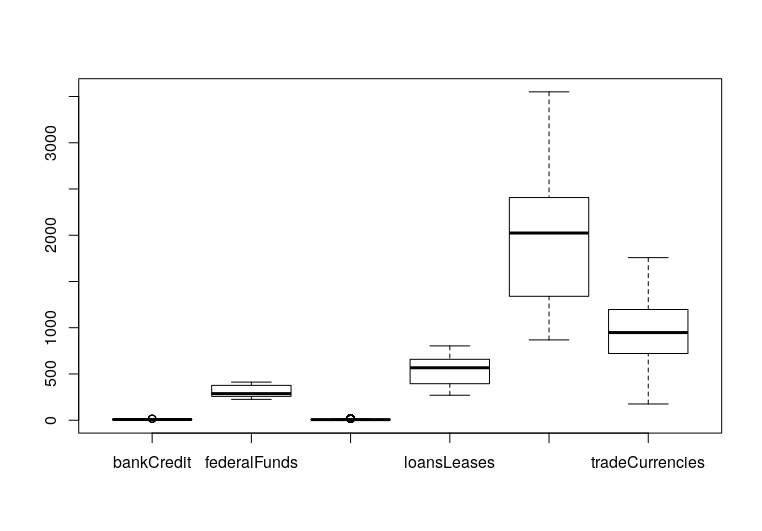
\includegraphics[scale=0.8]{./Imagenes/EDA/Regresion/boxplot_filtrado3.png}
	\caption{Boxplot manteniendo las variables seleccionadas.}
\end{figure}

Podemos ver que en las variables seleccionadas tenemos dos que poseen anomalías, vamos a estudiarlas en un boxplot aislado.

\begin{figure}[H]
	\centering
	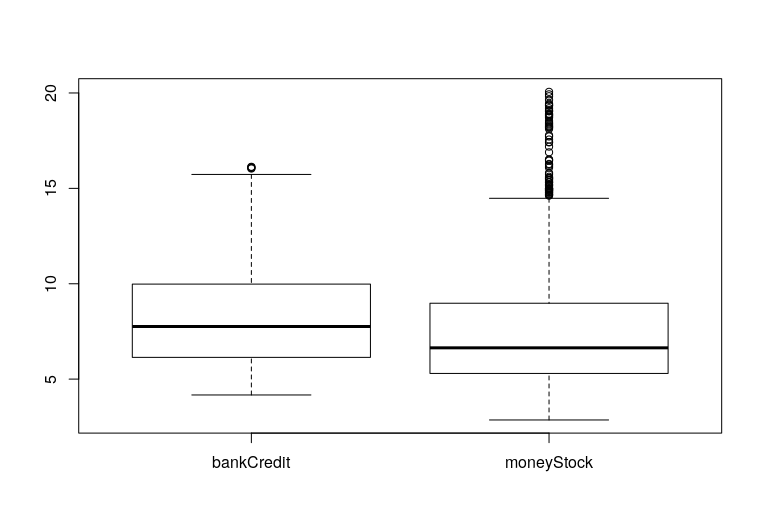
\includegraphics[scale=0.8]{./Imagenes/EDA/Regresion/boxplot_filtrado4.png}
	\caption{Boxplot de las variables que parecen tener anomalías.}
\end{figure}

Como podemos observar tenemos que la variable moneyStock tiene valores anómalos pero muy densos por lo que no debemos quitarlos. En el caso de bankCredit vamos a estudiar su scatterplot.

\begin{figure}[H]
	\centering
	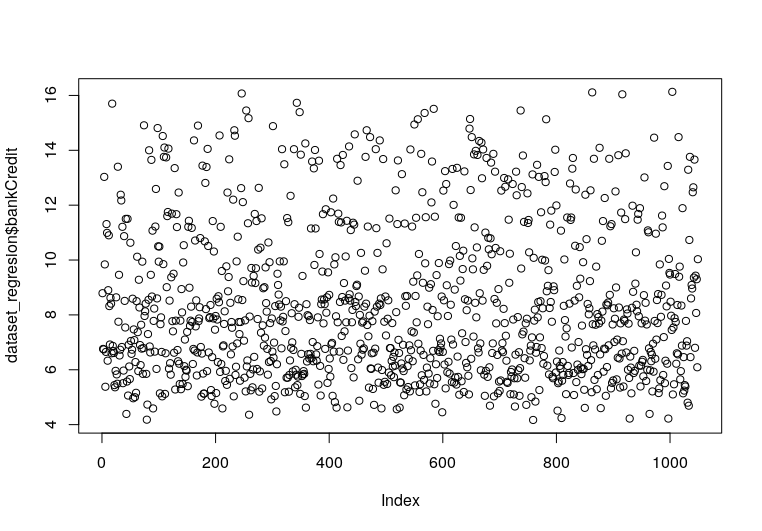
\includegraphics[scale=0.8]{./Imagenes/EDA/Regresion/scatterplot_bankCredit.png}
	\caption{ScatterPlot de la variable bankCredit}
\end{figure}

Podemos ver que las anomalías que nos encontramos no son tal pues es un conjunto distribuido de forma casi uniforme.

\subsubsection{Distribución de las variables}

Vamos a ver en primer lugar unos histogramas de las variables.

\begin{figure}[H]
	\centering
	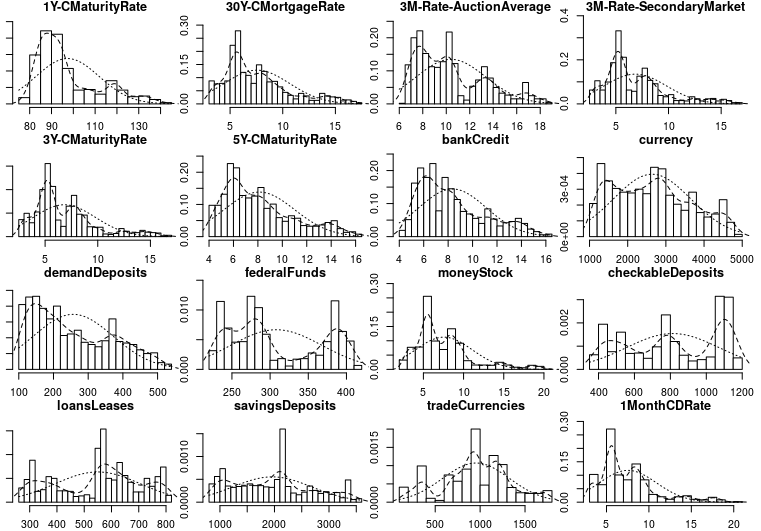
\includegraphics[scale=0.85]{./Imagenes/EDA/Regresion/histograma_todas.png}
	\caption{Histograma de todas las variables}
\end{figure}

Como podemos ver hemos acertado en el estudio previo de los estadísticos y podemos corroborar que la mayoría de variables tienen la cola derecha de su distribución más alargada. 

Podemos ver que las distribuciones no se parecen para nada a una normal de forma visual, aunque para poder estar seguros vamos a hacer un test de normalidad.

Para esto vamos a utilizar el test de Wilcoxon. Veamos los resultados.

\begin{figure}[H]
	\centering
	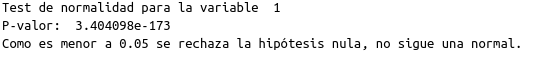
\includegraphics[scale=0.65]{./Imagenes/EDA/Regresion/test_normalidad1.png}
	\caption{Test de normalidad para la variable 1.}
\end{figure}

\begin{figure}[H]
	\centering
	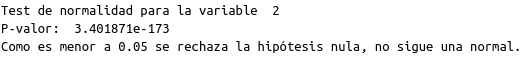
\includegraphics[scale=0.65]{./Imagenes/EDA/Regresion/test_normalidad2.png}
	\caption{Test de normalidad para la variable 2.}
\end{figure}
\begin{figure}[H]
	\centering
	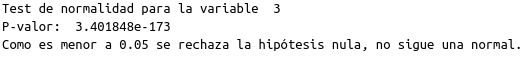
\includegraphics[scale=0.65]{./Imagenes/EDA/Regresion/test_normalidad3.png}
	\caption{Test de normalidad para la variable 3.}
\end{figure}

\begin{figure}[H]
	\centering
	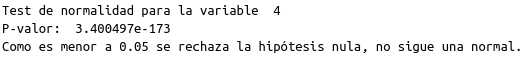
\includegraphics[scale=0.65]{./Imagenes/EDA/Regresion/test_normalidad4.png}
	\caption{Test de normalidad para la variable 4.}
\end{figure}

\begin{figure}[H]
	\centering
	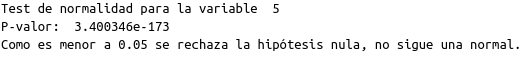
\includegraphics[scale=0.65]{./Imagenes/EDA/Regresion/test_normalidad5.png}
	\caption{Test de normalidad para la variable 5.}
\end{figure}

\begin{figure}[H]
	\centering
	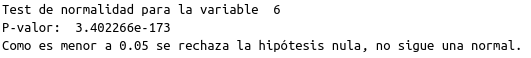
\includegraphics[scale=0.65]{./Imagenes/EDA/Regresion/test_normalidad6.png}
	\caption{Test de normalidad para la variable 6.}
\end{figure}

\begin{figure}[H]
	\centering
	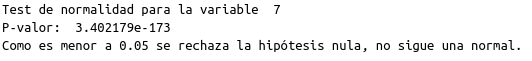
\includegraphics[scale=0.65]{./Imagenes/EDA/Regresion/test_normalidad7.png}
	\caption{Test de normalidad para la variable 7.}
\end{figure}

\begin{figure}[H]
	\centering
	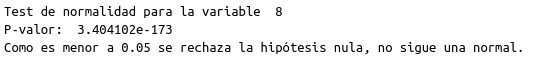
\includegraphics[scale=0.65]{./Imagenes/EDA/Regresion/test_normalidad8.png}
	\caption{Test de normalidad para la variable 8.}
\end{figure}

\begin{figure}[H]
	\centering
	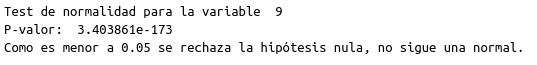
\includegraphics[scale=0.65]{./Imagenes/EDA/Regresion/test_normalidad9.png}
	\caption{Test de normalidad para la variable 9.}
\end{figure}

\begin{figure}[H]
	\centering
	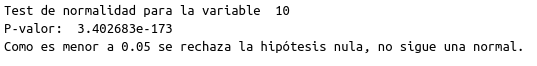
\includegraphics[scale=0.65]{./Imagenes/EDA/Regresion/test_normalidad10.png}
	\caption{Test de normalidad para la variable 10.}
\end{figure}

\begin{figure}[H]
	\centering
	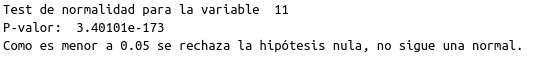
\includegraphics[scale=0.65]{./Imagenes/EDA/Regresion/test_normalidad11.png}
	\caption{Test de normalidad para la variable 11.}
\end{figure}

\begin{figure}[H]
	\centering
	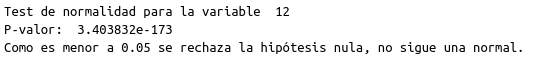
\includegraphics[scale=0.65]{./Imagenes/EDA/Regresion/test_normalidad12.png}
	\caption{Test de normalidad para la variable 12.}
\end{figure}

\begin{figure}[H]
	\centering
	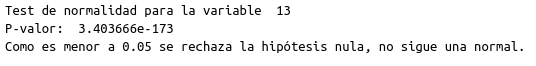
\includegraphics[scale=0.65]{./Imagenes/EDA/Regresion/test_normalidad13.png}
	\caption{Test de normalidad para la variable 13.}
\end{figure}

\begin{figure}[H]
	\centering
	\includegraphics[scale=0.65]{./Imagenes/EDA/Regresion/test_normalidad14.png}
	\caption{Test de normalidad para la variable 14.}
\end{figure}

\begin{figure}[H]
	\centering
	\includegraphics[scale=0.65]{./Imagenes/EDA/Regresion/test_normalidad15.png}
	\caption{Test de normalidad para la variable 15.}
\end{figure}

\begin{figure}[H]
	\centering
	\includegraphics[scale=0.65]{./Imagenes/EDA/Regresion/test_normalidad16.png}
	\caption{Test de normalidad para la variable 16.}
\end{figure}

Como podemos ver por los resultados del test podemos rechazar en todos los casos la hipótesis nula por lo que podemos decir que ninguna de las variables sigue una distribución normal, tal y como hemos podido ver de forma gráfica.


\subsection{Conjunto de Clasificación}

El conjunto con el que vamos a atacar el problema de clasificación es el conjunto de datos ``heart''. Vamos a analizar este conjunto de datos antes de abordar el problema.

El problema dispone de 14 variables, siendo la última la clase a la que pertenece cada instancia.

Vamos a ver los tipos de las variables.

\begin{figure}[H]
	\centering
	\includegraphics[scale=0.7]{./Imagenes/EDA/Clasificacion/tipos_variables.png}
	\caption{Tipos de las variables.}
\end{figure}

Podemos observar que todas las variables son de tipo integer, es decir, de tipo entero y que hay una variable de tipo numeric, o lo que es lo mismo, de tipo real.

Vamos a realizar el estudio del conjunto completo dividiéndolo en dos partes, la variable que nos indica la clase y el resto de variables.

\subsubsection{Estudio de los estadísticos}

\subsubsection*{Salida}

Vamos a ver los estadísticos que nos da la variable de salida o lo que es lo mismo, la clase asociada a cada instancia.

\begin{figure}[H]
	\centering
	\includegraphics[scale=0.7]{./Imagenes/EDA/Clasificacion/estadisticos_class.png}
	\caption{Estadísticos de la variable de salida.}
\end{figure}

Para poder analizar los estadísticos de esta variable tenemos que tener en cuenta que es una variable que sólo tiene dos posibles valores: 1 y 2. 

La media es $1.444444$ por lo que podemos decir que seguramente encontraremos un número mayor de instancias de la clase 1 que de la clase 2, pues si fuera al contrario la media debería ser más grande que $1.5$. Este hecho es también contrastable por el valor de la moda, o lo que es lo mismo, el valor más frecuente. La moda es $1$ por lo que ya sabemos que hay más instancias de la clase 1 que de la 2. En este caso estudiar la distribución carece de sentido por tomar únicamente dos valores, por lo que no estudiaremos la asimetría ni la curtosis.

\subsubsection*{Variable 1: Age}

Vamos a estudiar los estadísticos que nos arroja la variable.

\begin{figure}[H]
	\centering
	\includegraphics[scale=0.7]{./Imagenes/EDA/Clasificacion/estadisticos_variable1.png}
	\caption{Estadísticos de la variable 1.}
\end{figure}

En primer lugar cabe decir que esta variable es de tipo entero. Podemos ver que el intervalo en el que se mueven los valores es $[29,77]$. 

Como podemos ver la media, la mediana y la moda están muy próximas entre sí por lo que la distribución debe estar centrada. Este hecho se puede contrastar con el coeficiente de asimetría que aunque es negativo está muy cercano a $0$ lo que nos indica que la distribución es prácticamente simétrica.

En cuanto a la curtosis podemos ver que es negativa por lo que la distribución es más achatada que su normal homóloga en parámetros.

\subsubsection*{Variable 2: Sex}

Vamos a estudiar los estadísticos que nos arroja la variable.

\begin{figure}[H]
	\centering
	\includegraphics[scale=0.7]{./Imagenes/EDA/Clasificacion/estadisticos_variable2.png}
	\caption{Estadísticos de la variable 2.}
\end{figure}

Esta variable es de tipo entero y sólo puede tomar dos valores: $0$ y $1$, siendo cada uno de los números el sexo masculino o femenino. Podemos ver que la media es $0.6777778$ por lo que hay más valores de $1$ que de $0$ y por tanto debe haber un género predominante sobre el otro dentro de los datos.

Al ser una variable que sólo puede tomar dos valores no tiene sentido que estudiemos la distribución de la variable.

\subsubsection*{Variable 3: ChestPainType}

Vamos a estudiar los estadísticos que nos arroja la variable.

\begin{figure}[H]
	\centering
	\includegraphics[scale=0.7]{./Imagenes/EDA/Clasificacion/estadisticos_variable3.png}
	\caption{Estadísticos de la variable 3.}
\end{figure}

Esta variable es de tipo entero y toma valores en el intervalo $[1,4]$ indicando el tipo de dolor de pecho que posee el paciente. La media y la mediana no tienen sentido en este caso pues no son fácilmente interpretables. Al no ser algo binario no podemos establecer en qué grado aparece un valor sobre otro.

Lo que si nos puede ser útil de analizar es la moda. Podemos ver que toma valor $4$, o lo que es lo mismo, el dolor de pecho más típico es aquel que va asociado con el número $4$.

Algo que sí podemos decir sobre esta variable es que está desplazada hacia la derecha y debería de tener una cola más pesada a la derecha y más alargada a la izquierda. Esto lo podemos intuir pues la desviación típica es cercana a $1$ y por tanto el intervalo que contiene el 95\% de los datos debería de ser $[1,5]$ aproximadamente, por lo que vemos que está desplazada a la derecha con respecto al intervalo $[1,4]$.

Este dato es comprobable también por el coeficiente de asimetría que es negativo y por tanto nos indica que la distribución es asimétrica a la izquierda. En cuanto a la curtosis podemos ver que es negativa y por tanto la distribución debe ser algo más achatada que una distribución normal de mismos parámetros.

\subsubsection*{Variable 4: RestBloodPressure}

Vamos a estudiar los estadísticos que nos arroja la variable.

\begin{figure}[H]
	\centering
	\includegraphics[scale=0.7]{./Imagenes/EDA/Clasificacion/estadisticos_variable4.png}
	\caption{Estadísticos de la variable 4.}
\end{figure}

Esta es también una variable de tipo entero. Podemos ver que toma valores en el intervalo $[94, 200]$. La media y la mediana están muy próximas entre sí por lo que podemos pensar que la distribución está centrada. Por contra si miramos la moda es de $120$ por lo que podemos intuir una asimetría en la distribución.

Si miramos el coeficiente de asimetría tenemos que es positivo por lo que la distribución es asimétrica a la derecha. Esto nos indica que la cola de la derecha es algo más alargada que la de la izquierda. En cuanto a la curtosis podemos ver que es positiva por lo que la distribución es más apuntada que su distribución normal asociada de mismos parámetros.

\subsubsection*{Variable 5: SerumCholestoral}

Vamos a estudiar los estadísticos que nos arroja la variable.

\begin{figure}[H]
	\centering
	\includegraphics[scale=0.7]{./Imagenes/EDA/Clasificacion/estadisticos_variable5.png}
	\caption{Estadísticos de la variable 5.}
\end{figure}

Esta variable también es de tipo entero. El intervalo en el que toma valores es $[126,564]$. Si observamos la media y la mediana están próximas, por contra la moda es significativamente menor que ambas por lo que nos puede dar a intuir una asimetría derecha con una cola de la distribución algo más alargada.

Este hecho viene dado por el coeficiente de asimetría. Como podemos ver es positivo y además lo suficientemente grande como para que podamos decir que la asimetría es notable. Este hecho puede no ser tan sencillo de deducir a partir de los datos porque la variable es de tipo entero. Esto puede hacer que haya algunos valores más frecuentes que otros y por tanto la asimetría no sea tan evidente a través de los estadísticos básicos. 

Otro valor muy significativo es la curtosis que podemos ver que es positiva y muy grande, lo que nos está indicando que la distribución es extremadamente puntiaguda y por tanto podemos pensar que el argumento anterior (hay valores mucho más frecuentes que otros) es algo a tener en cuenta.

\subsubsection*{Variable 6: FastingBloodSugar}

Vamos a estudiar los estadísticos que nos arroja la variable.

\begin{figure}[H]
	\centering
	\includegraphics[scale=0.7]{./Imagenes/EDA/Clasificacion/estadisticos_variable6.png}
	\caption{Estadísticos de la variable 6.}
\end{figure}

La variable FastingBloodSugar es de tipo entero y sólo puede tomar dos valores: $0$ y $1$. Si vemos la media tenemos que es $0.1481481$ por lo que podemos decir que hay muchas más instancias que toman valor $0$ frente a las que toman valor $1$. El equilibrio, es decir si hubiera el mismo número de $0$ que de $1$, sería $0.5$ por lo que podemos ver el desequilibrio de valores. La moda es $0$ también por lo que corroboramos que este es el valor más frecuente.

En cuanto a la curtosis y asimetría no nos aportan más información que la ya razonada pues estamos ante una variable binaria.

\subsubsection*{Variable 7: ResElectrocardiographic}

Vamos a estudiar los estadísticos que nos arroja la variable.

\begin{figure}[H]
	\centering
	\includegraphics[scale=0.7]{./Imagenes/EDA/Clasificacion/estadisticos_variable7.png}
	\caption{Estadísticos de la variable 7.}
\end{figure}

Esta variable es también de tipo entero y podemos ver que toma valores en el intervalo $[0,2]$ por lo que sólo puede tomar los valores $0$, $1$ y $2$.La media es cercana a $1$ por lo que pueden pasar dos cosas con los valores de esta variable: la primera es que los valores que toman las 3 variables estén equilibrados y la segunda es que las ocurrencias de $0$ y $2$ estén equilibradas.

La moda es 2, cosa que podemos ver pues la media es ligeramente superior a $1$. Como tenemos una variable muy simple (sólo toma tres valores) el coeficiente de asimetría no nos da más información que la media, pudiendo corroborar que la distribución es simétrica. En cuanto a la curtosis podemos  ver que es mucho más achatada que su distribución normal asociada, por lo que podemos intuir que habrá menos ocurrencias del valor $1$ frente al $0$ y $2$.

\subsubsection*{Variable 8: MaxHeartRate}

Vamos a estudiar los estadísticos que nos arroja la variable.

\begin{figure}[H]
	\centering
	\includegraphics[scale=0.7]{./Imagenes/EDA/Clasificacion/estadisticos_variable8.png}
	\caption{Estadísticos de la variable 8.}
\end{figure}

La variable MaxHeartRate es de tipo entero. Podemos ver que toma valores en el intervalo $[71,202]$. La media y la mediana están razonablemente cercanas pero la moda es sustancialmente mayor a ambas, lo que nos está indicando que la cola izquierda debe ser algo más alargada que la derecha. Esto podríamos intentar razonarlo también calculando el intervalo en el que deberíamos encontrar el 95\% de los datos ($[103.34636,196.00924]$) pero en este caso no nos otorga mucha información.

El coeficiente de asimetría es negativo lo que nos indica una asimetría a la izquierda. La curtosis es negativa pero muy cercana a $0$ por lo que podemos decir que la distribución estará ligeramente achatada.

\subsubsection*{Variable 9: ExerciseInduced}

Vamos a estudiar los estadísticos que nos arroja la variable.

\begin{figure}[H]
	\centering
	\includegraphics[scale=0.7]{./Imagenes/EDA/Clasificacion/estadisticos_variable9.png}
	\caption{Estadísticos de la variable 9.}
\end{figure}

Esta variable es también de tipo entero y podemos ver que toma valores en el intervalo $[0,1]$ por lo que es binaria. La media es menor que $0.5$ lo que nos indica que hay más ocurrencias del valor $0$ que del valor $1$, cuestión que se refuerza al ver que la mediana y la moda son $0$.

En cuanto a la curtosis y el coeficiente de asimetría carecen de sentido al no aportar mayor infomación en una variable binaria.

\subsubsection*{Variable 10: Oldpeak}

Vamos a estudiar los estadísticos que nos arroja la variable.

\begin{figure}[H]
	\centering
	\includegraphics[scale=0.7]{./Imagenes/EDA/Clasificacion/estadisticos_variable10.png}
	\caption{Estadísticos de la variable 10.}
\end{figure}

Esta es la única variable del conjunto de datos que es de tipo real. Toma valores dentro del intervalo $[0,62]$ y podemos ver que la media es $8.9$. La mediana es tan solo $4$ por lo que podemos intuir que la cola derecha será muy alargada comparado con la izquierda. En cuanto a la moda podemos ver que el valor más frecuente es $0$.

Si estudiamos la curtosis y asimetría podemos ver que la distribución es muy asimétrica a la derecha, lo que sustenta el razonamiento de la cola derecha más alargada. La curtosis es positiva y muy grande por lo que podemos ver que la distribución es mucho más puntiaguda o apuntada que la distribución de una normal de mismos parámetros.

\subsubsection*{Variable 11: Slope}

Vamos a estudiar los estadísticos que nos arroja la variable.

\begin{figure}[H]
	\centering
	\includegraphics[scale=0.7]{./Imagenes/EDA/Clasificacion/estadisticos_variable11.png}
	\caption{Estadísticos de la variable 11.}
\end{figure}

La variable Slope es de tipo entero y toma valores dentro del intervalo $[1,3]$, por lo que sólo puede tomar $3$ valores distintos: $1$, $2$, y $3$. La media es $1.585185$ lo que nos indica que hay una descompensación hacia el $1$ teniendo más ocurrencias de éste valor.

Este hecho lo podemos contrastar con el valor de la moda que es $1$. En cuanto a la mediana podemos ver que es $2$ lo que nos hace pensar que aproximadamente puede haber el mismo número de ocurrencias del valor $1$ que de los valores $2$ y $3$ juntos.

El coeficiente de asimetría soporta estos razonamientos, pues es positivo indicándonos que la cola derecha es más alargada que la izquierda. En cuanto a la curtosis podemos ver que es negativa indicando que la distribución es más achatada que una normal de mismos parámetros.

\subsubsection*{Variable 12: MajorVessels}

Vamos a estudiar los estadísticos que nos arroja la variable.

\begin{figure}[H]
	\centering
	\includegraphics[scale=0.7]{./Imagenes/EDA/Clasificacion/estadisticos_variable12.png}
	\caption{Estadísticos de la variable 12.}
\end{figure}

Esta variable es de tipo entero y toma valores en el intervalo $[0,3]$, por lo que sólo puede tomar $4$ valores distintos. Podemos ver que la media está entre $0$ y $1$ lo que nos lleva a pensar que debe haber más ocurrencias de valores $0$ que del resto. La moda y la mediana corroboran esta suposición. 

La asimetría es positiva, lo que nos indica que la cola derecha debe ser más alargada que la izquierda. Por otro lado la curtosis es positiva pero no muy grande por lo que la distribución es ligeramente más apuntada que una normal de mismos parámetros.

\subsubsection*{Variable 13: Thal}

Vamos a estudiar los estadísticos que nos arroja la variable.

\begin{figure}[H]
	\centering
	\includegraphics[scale=0.7]{./Imagenes/EDA/Clasificacion/estadisticos_variable13.png}
	\caption{Estadísticos de la variable 13.}
\end{figure}

La variable Thal es de tipo entero también y toma valores en el intervalo $[3,7]$. La media es $4.696296$ y la mediana y la moda $3$. Esto nos deja pensar que la distribución será aproximadamente simétrica pues no se percibe por estos estadísticos un desbalanceo acusado. El coeficiente de asimetría, aunque positivo, posee un valor muy cercano a cero. Por otro lado la curtosis es negativa y por tanto es más achatada que su distribución normal homóloga.

\subsubsection{Estudio de la correlación de las variables}

Vamos a estudiar la correlación entre variables por si puediéramos encontrar, como en el caso del conjunto de regresión, variables altamente correladas que se puedan eliminar.

Veamos la correlación entre las variables:

\begin{figure}[H]
	\centering
	\includegraphics[scale=0.7]{./Imagenes/EDA/Clasificacion/correlacion_entre_variables1.png}
	\caption{Correlación entre las variables sin contar la de clase.}
\end{figure}

\begin{figure}[H]
	\centering
	\includegraphics[scale=0.7]{./Imagenes/EDA/Clasificacion/correlacion_entre_variables2.png}
	\caption{Correlación entre las variables sin contar la de clase.}
\end{figure}

Como podemos observar no hay ninguna variable altamente correlada con otra, por lo que no podemos simplificar el conjunto de datos.

Este hecho puede venir de que la mayoría de variables son de tipo entero con muy pocos valores a tomar.

Veamos ahora la correlación entre las variables con la variable de clase.

\begin{figure}[H]
	\centering
	\includegraphics[scale=0.7]{./Imagenes/EDA/Clasificacion/correlacion_salida.png}
	\caption{Correlación entre las variables con la de clase.}
\end{figure}

Podemos ver que no hay variables con un alto grado de correlación con la salida. Tendremos que comprobar con el ajuste de los modelos de clasificación el desempeño que obtenemos.

\subsubsection{Valores perdidos}

Vamos a comprobar si nuestro conjunto de clasificación tiene algún valor perdido o estamos ante un conjunto limpio de missing values como en el caso de regresión.

\begin{figure}[H]
	\centering
	\includegraphics[scale=0.7]{./Imagenes/EDA/Clasificacion/valores_perdidos.png}
	\caption{Valores perdidos en el conjunto de clasificación}
\end{figure}

Como podemos ver tenemos un conjunto sin valores perdidos, por lo que no tenemos que hacer mayores disquisiciones en este terreno.

\subsubsection{Outliers}



\subsubsection{Distribución de las variables}



\end{document}